\documentclass[11pt]{amsart}
\usepackage[a4paper,margin=2.7cm]{geometry}
\usepackage{amssymb}
\usepackage{tikz}
\usepackage{booktabs}
\usepackage[hidelinks]{hyperref}

\newtheorem{theorem}{Theorem}
\newtheorem{lemma}{Lemma}
\newtheorem{proposition}[lemma]{Proposition}
\theoremstyle{remark}
\newtheorem{remark}{Remark}

\title[Fences and orbits of linear extensions]{Fences do not maximise orbits of linear extensions}
\author{Vamshi Jandhyala}
\date{Preprint, version 1, 23 October 2026. Not peer reviewed.}
\subjclass[2020]{06A07, 05A05, 05A16}
\keywords{poset, linear extension, automorphism group, fence, alternating permutation}

\begin{document}

\begin{abstract}
For a finite poset $P$ let $f(P)=e(P)/\#\mathrm{Aut}(P)$ be the number of orbits of the automorphism group on the linear extensions, and let $g(n)$ be the largest value of $f$ over $n$-element posets. Stanley asked what can be said about $g(n)$ and whether the maximisers are disjoint unions of fences. By exhaustive computation we find $g(n)$ and all maximisers for $n\le11$: fence unions are maximisers exactly for $n\le7$ and $n=9$, and the first failure is an eight-element poset with $f=2384$ against $2100$ for the best fence union. We also prove that for every $n\ge58$ no maximiser is a union of fences. The proof combines a construction posted by Graham with an upper bound for fence unions: a poset with $t$ disjoint comparable pairs has at most $n!/2^t$ linear extensions.
\end{abstract}

\maketitle

\noindent\emph{Status of this preprint.} This version has not yet been independently reviewed.

\section{Introduction}

A linear extension of a finite poset $P$ is a way of listing its elements so that every relation $x<y$ puts $x$ before $y$. The automorphism group of $P$ permutes these listings, and only the identity fixes one, so every orbit has exactly $\#\mathrm{Aut}(P)$ elements. The number of orbits is therefore
\[
f(P)=\frac{e(P)}{\#\mathrm{Aut}(P)},
\]
where $e(P)$ is the number of linear extensions. Large $e(P)$ wants few relations, but few relations bring symmetry: the antichain has $e=n!$ and $f=1$. Stanley~\cite{MO} asked how large $f$ can be. Writing $g(n)$ for the maximum over $n$-element posets, what can be said about $g(n)$ and the posets attaining it, and in particular, are they disjoint unions of fences?

A \emph{fence} $Z_m$ is the poset $x_1<x_2>x_3<x_4>\cdots$ on $m$ elements; for odd $m\ge3$ its dual is a different poset, and we count both as fences. A linear extension of $Z_m$ gives positions $L(x_1)<L(x_2)>L(x_3)<\cdots$, which is an alternating permutation, so $e(Z_m)=E_m$, the Euler zigzag number~\cite{St}. Fences are a natural guess: they have many linear extensions for the number of relations, and little symmetry.

\emph{A first case.} For $n=5$ the maximiser is $Z_4+\bullet$, a four-element fence and a separate point: $e=5\cdot E_4=25$ and the automorphism group is trivial, so $f=25$. At $n=8$ this pattern breaks. The best union of fences is $Z_2+Z_4+2\bullet$, with $e=4200$ and two automorphisms (swap the points), so $f=2100$. The poset $Q+\bullet$ of Figure~\ref{fig:Q}, a six-element fence with one extra element below its middle peak, plus a point, has $e=8\cdot298=2384$ and no automorphisms.

\begin{figure}[ht]
\centering
\begin{tikzpicture}[scale=0.8,every node/.style={circle,fill,inner sep=1.6pt}]
  \node[label=below:$a$] (a) at (0,0) {}; \node[label=above:$b$] (b) at (1,1.2) {};
  \node[label=below:$c$] (c) at (2,0) {}; \node[label=above:$d$] (d) at (3,1.2) {};
  \node[label=below:$e$] (e) at (4,0) {}; \node[label=above:$f$] (f) at (5,1.2) {};
  \node[label=below:$g$] (g) at (3,-0.6) {};
  \draw (a)--(b)--(c)--(d)--(e)--(f); \draw (g)--(d);
  \node (p) at (6.3,0.6) {};
  \node[draw=none,fill=none] at (2.5,-1.6) {$Q+\bullet$: $f=2384$};
  \begin{scope}[xshift=8.6cm]
  \node (a2) at (0,0) {}; \node (b2) at (1,1.2) {};
  \node (c2) at (2,0) {}; \node (d2) at (3,1.2) {};
  \node (p1) at (4.2,0.6) {}; \node (p2) at (5,0.6) {};
  \node (u) at (5.9,0) {}; \node (v) at (5.9,1.2) {};
  \draw (a2)--(b2)--(c2)--(d2); \draw (u)--(v);
  \node[draw=none,fill=none] at (3,-1.6) {$Z_4+Z_2+2\bullet$: $f=2100$};
  \end{scope}
\end{tikzpicture}
\caption{Eight elements. Left: the maximiser $Q+\bullet$ (and its dual), not a union of fences, since $d$ is comparable with three elements. Right: the best union of fences. The extra element $g$ adds relations but removes the reflection of the fence, and that trade wins.}
\label{fig:Q}
\end{figure}

\begin{theorem}\label{thm:small}
For $n\le11$ the values of $g(n)$ are
\[
1,\ 1,\ 3,\ 6,\ 25,\ 75,\ 525,\ 2384,\ 15372,\ 107280,\ 798435 .
\]
A disjoint union of fences attains $g(n)$ exactly when $n\le7$ or $n=9$. The maximisers for $n=8,10,11$ are $Q+\bullet$, $Q+Z_2+\bullet$ and $R+Z_2+\bullet$ (with the duals of the first two), where $R$ is $Q$ with one more element above $c$.
\end{theorem}

Theorem~\ref{thm:small} is a finite computation (Section~\ref{sec:comp}). The second result settles the fence question for all large $n$.

\begin{theorem}\label{thm:large}
For every $n\ge58$, no poset attaining $g(n)$ is a disjoint union of fences.
\end{theorem}

The lower bound comes from Graham's answer~\cite{Gr} to Stanley's question: a few maximal elements over many minimal ones, wired so that the only symmetry permutes the top. Graham estimated that this beats tree-like posets for large $n$. The new ingredient is a bound that makes the comparison with fences rigorous and explicit (Proposition~\ref{prop:fence}); for $58\le n\le180$ it is completed by an exact computation of the best fence union. Between $12$ and $57$ the question stays open.

\section{An upper bound for unions of fences}

The bound rests on one counting fact.

\begin{lemma}\label{lem:pairs}
If $P$ has $n$ elements and contains $t$ pairwise disjoint pairs $a_i<b_i$, then $e(P)\le n!/2^t$.
\end{lemma}

\begin{proof}
Order the elements uniformly at random. For disjoint pairs the events ``$a_i$ comes before $b_i$'' are independent, each of probability $\tfrac12$, so all $t$ hold for exactly $n!/2^t$ orderings. Every linear extension is one of them.
\end{proof}

In words: each disjoint relation at least halves the number of admissible orderings. A fence $Z_m$ contains the $\lfloor m/2\rfloor$ disjoint pairs $x_1<x_2$, $x_3<x_4$, \dots, and $\lfloor m/2\rfloor\ge m/3$ when $m\ge2$.

\begin{proposition}\label{prop:fence}
Let $P$ be a disjoint union of fences on $n$ elements, $k$ of which are isolated points. Then
\[
f(P)\le\frac{n!}{2^{(n-k)/3}\,k!} .
\]
\end{proposition}

\begin{proof}
The non-singleton fences cover $n-k$ elements and contain at least $(n-k)/3$ disjoint comparable pairs, so $e(P)\le n!/2^{(n-k)/3}$ by Lemma~\ref{lem:pairs}. Any permutation of the $k$ isolated points is an automorphism, so $\#\mathrm{Aut}(P)\ge k!$.
\end{proof}

The bound reads: a union of fences loses a factor $2^{1/3}$ per element in a fence, and a factor $k!$ for its isolated points. Whatever $k$ is, the combined loss is at least $2^{(n-1)/3}$, exponential in $n$ (Section~4). The construction below loses only a factor $n^{\log_2n+1}$, which grows more slowly than any exponential.

For the exact comparison in the middle range we also need the exact value. The components of a fence union are fences $Z_m$ and, for odd $m\ge3$, their duals $Z_m^*$. One has $\#\mathrm{Aut}(Z_m)=2$ for odd $m\ge3$ (the reflection $x_i\mapsto x_{m+1-i}$) and $1$ otherwise, since an automorphism of a path is the identity or the reflection, and for even $m$ the reflection reverses the relations. For a union with $c$ copies of a component $C$ of size $m$, the standard shuffle and wreath-product counts give
\begin{equation}\label{eq:exact}
f(P)=n!\prod_{C}\frac{1}{c_C!}\Bigl(\frac{E_m}{m!\,\#\mathrm{Aut}(C)}\Bigr)^{c_C}.
\end{equation}
Each component contributes its share $E_m/m!$ of orderings, divided by its own symmetry, and $c$ identical components contribute a further $c!$ for permuting them. Maximising~\eqref{eq:exact} over multisets of components is a knapsack over $n$, computed exactly in rational arithmetic.

\section{Graham's construction}

\begin{lemma}[Graham~\cite{Gr}]\label{lem:graham}
Let $j\ge1$ and $1\le m\le2^j-1$. There is a poset on $n=j+m$ elements with $f\ge m!$.
\end{lemma}

\begin{proof}
Take $j$ top elements $A$ and $m$ bottom elements $b_S$, one for each set $S$ in a family of $m$ distinct nonempty subsets of $A$ that contains $A$ itself, with $b_S<a$ exactly when $a\in S$. Listing all bottoms first, in any order, and then all tops, in any order, gives $m!\,j!$ linear extensions. Each bottom lies below some top and each top lies above $b_A$, so bottoms are exactly the minimal elements that are not maximal, and every automorphism maps tops to tops. An automorphism is determined by its action on $A$, because $b_S$ is the only bottom whose up-set is $S$. So $\#\mathrm{Aut}\le j!$ and $f\ge m!$.
\end{proof}

What pins down the tops is that $A$ itself is one of the sets: every top then lies above $b_A$. The empty set could be allowed too (an isolated bottom $b_\emptyset$ is still minimal and still the only bottom with its up-set, and the Lean proof does without the nonempty condition), but nothing is gained for Theorem~\ref{thm:large}. Figure~\ref{fig:graham} shows a small case.

\begin{figure}[ht]
\centering
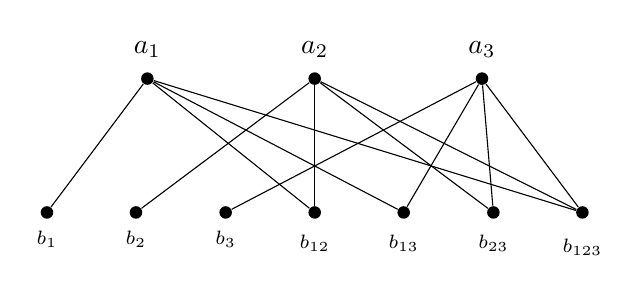
\begin{tikzpicture}[scale=0.85,every node/.style={circle,fill,inner sep=1.6pt}]
  \foreach \i/\x in {1/1.5,2/4,3/6.5} { \node[label=above:$a_\i$] (a\i) at (\x,2) {}; }
  \foreach \k/\S/\x in {1/{1}/0,2/{2}/1.33,3/{3}/2.67,4/{12}/4,5/{13}/5.33,6/{23}/6.67,7/{123}/8} { \node[label=below:{\scriptsize $b_{\S}$}] (b\k) at (\x,0) {}; }
  \draw (b1)--(a1); \draw (b2)--(a2); \draw (b3)--(a3);
  \draw (b4)--(a1); \draw (b4)--(a2); \draw (b5)--(a1); \draw (b5)--(a3);
  \draw (b6)--(a2); \draw (b6)--(a3); \draw (b7)--(a1); \draw (b7)--(a2); \draw (b7)--(a3);
\end{tikzpicture}
\caption{Graham's construction with $j=3$ tops and all $m=7$ nonempty subsets as bottoms ($n=10$). Any order of the seven bottoms followed by any order of the three tops is a linear extension, so $e\ge7!\,3!$, while the only symmetries permute the tops, so $\#\mathrm{Aut}\le3!$ and $f\ge7!=5040$. For larger $n$ the bottoms outnumber the tops exponentially, and $f$ is within a factor $n^{\log_2n+1}$ of $n!$.}
\label{fig:graham}
\end{figure}

For given $n$ let $J(n)$ be the least $j$ with $2^j+j-1\ge n$; then $g(n)\ge(n-J(n))!$. Since $J(n)\le\log_2n+1$, this is $n!$ divided by a factor at most $n^{\log_2n+1}$.

\section{Proof of Theorem~\ref{thm:large}}

Fix $n$ and a union of fences $P$ with $k$ isolated points; put $j=J(n)$. It is enough to show $f(P)<(n-j)!$.

\emph{Large $n$.} By Proposition~\ref{prop:fence} it suffices that $k!\,2^{(n-k)/3}>n!/(n-j)!$ for every $k$. The left side is smallest at $k\in\{0,1\}$, where it is at least $2^{(n-1)/3}$, because each further step multiplies it by $(k+1)\,2^{-1/3}\ge1$. So it suffices that
\begin{equation}\label{eq:cube}
\Bigl(\frac{n!}{(n-j)!}\Bigr)^3<2^{\,n-1}.
\end{equation}
The left side is at most $n^{3j}\le n^{3(\log_2n+1)}$, and $(n-1)/3>(\log_2n+1)\log_2n$ holds at $n=200$ and its difference grows with $n$, so~\eqref{eq:cube} holds for all $n\ge200$. Checking~\eqref{eq:cube} exactly with integers shows it holds for every $181\le n\le199$ as well (and fails at $n=180$).

\emph{Middle range.} For $58\le n\le180$ we compute the exact maximum of~\eqref{eq:exact} over all fence unions on $n$ points and compare it with $(n-J(n))!$; the construction wins at every $n$ in this range. For $12\le n\le57$ it loses at every $n$, so this argument says nothing there. \qed

\section{The computation behind Theorem~\ref{thm:small}}\label{sec:comp}

Every poset on at most $11$ elements was generated by nauty's \texttt{genposetg}~\cite{McK} ($46{,}749{,}427$ posets at $n=11$; the counts for $n\le11$ match OEIS A000112). For each, $e(P)$ was computed by dynamic programming over down-sets and $\#\mathrm{Aut}(P)$ by backtracking over the Hasse diagram. Integrality of $e(P)/\#\mathrm{Aut}(P)$ was asserted for every poset, as the free action requires. For $n\le8$ the whole search was repeated independently in Sage, with the same maxima and maximisers. The best fence unions for $n\le11$, from~\eqref{eq:exact}, agree with $g(n)$ exactly when $n\le7$ or $n=9$, and are $2100$, $76860$ and $704550$ for $n=8,10,11$.

\begin{remark}
The sequence $g(n)$ is not in the OEIS (searched 23 October 2026). Lemma~\ref{lem:graham} and the bound $f(P)\le e(P)\le n!$ give $n!/n^{\log_2n+1}\le g(n)\le n!$. Whether fence unions ever maximise for $12\le n\le57$ is open; the computed maximisers suggest that a fence with pendant elements, as in $Q$ and $R$, is the competitor to beat in that range.
\end{remark}

\emph{Verification.} The accompanying repository contains the search programs for $n\le11$ with the Sage cross-check; an exact computation of the best fence union for every $n\le200$ with two independent programs that share no code; brute-force checks of $e(Z_m)=E_m$ and of $\#\mathrm{Aut}(Z_m)$ for $m\le8$; and an exact check of~\eqref{eq:cube}. In Lean~4 with Mathlib are formalised: the free action and $f=e/\#\mathrm{Aut}$; the posets $Q$, $Q+\bullet$, $R$ and their counts; Lemma~\ref{lem:pairs}, Proposition~\ref{prop:fence}, Lemma~\ref{lem:graham}, and Theorem~\ref{thm:large} for $n\ge181$. The exhaustive search and the range $58\le n\le180$ are computations.

\emph{Acknowledgement.} The question is due to Richard Stanley and the construction of Lemma~\ref{lem:graham} to Graham's MathOverflow answer. The computations, the proofs and this note were developed with Claude (Anthropic), which also wrote the Lean formalisation.

\begin{thebibliography}{9}
\bibitem{Gr} Graham (MathOverflow user), answer to~\cite{MO}, \url{https://mathoverflow.net/a/516180}, 19 October 2026, accessed 23 October 2026.
\bibitem{McK} B.~D.~McKay, nauty and Traces, \url{https://pallini.di.uniroma1.it}, \texttt{genposetg}, accessed 23 October 2026.
\bibitem{MO} R.~P.~Stanley, Maximizing the number of orbits of linear extensions of a poset, MathOverflow question 516140 (2026), \url{https://mathoverflow.net/q/516140}, accessed 23 October 2026.
\bibitem{St} R.~P.~Stanley, A survey of alternating permutations, in \emph{Combinatorics and Graphs}, Contemp. Math. \textbf{531}, Amer. Math. Soc., 2010. arXiv:0912.4240.
\end{thebibliography}

\end{document}
